%----------------------------------------------------------------------------------------
%----------------------------------------------------------------------------------------
%----------------------------------------------------------------------------------------
%Result Part 1: 1D SOMs
%----------------------------------------------------------------------------------------
%----------------------------------------------------------------------------------------
%----------------------------------------------------------------------------------------
\section{One dimensional self-organizing maps}
    \label{Sec: 1d_cluster}
%Why 1D maps are useful
    The purpose of  exploring the M31 data with 1D maps is to monitor the general behaviour of data. 
    One-dimensional SOMs can have the minimum number of clusters, $1\times2$, up to the highest number of clusters possible.
    In a small sample like ours, smaller grid SOMs are very useful to find correlations that cannot be found without  clustering the data.
    On the other hand, larger grid 1D SOMs are a helpful tool to get quick insight into the data.
%    In the following section, we are going to show how we used 1D SOMs to extract information from available data in M31.
%Clustering
 %   \subsection{Clustering M31 data}

        In order to monitor how the data behaves, we created SOMs with two to fourteen neurons (Fig.~\ref{fig: M31_nets_1d}).
        The $1\times2$ network (Fig.~\ref{fig: M31_net_1by2}) shows how the M31 data can be divided into two broad categories.
        The $1\times14$ network (Fig.~\ref{fig: M31_net_1by14}) is the first network in which all the regions in M31 are completely separated.
        Since in the higher network sizes, regions have more space to be separated based on their differences,  going from the $1\times2$ to the $1\times14$ network the distance between M31 regions increases, until they are completely separated. 
        
      Fig.~\ref{fig: M31_net_1by2} shows that by forcing the regions in the M31 to be divided into two groups, regions 1, 2, 9 and 10 occupy one neuron and the other regions occupy the other one.
        The medium grey colour between two neurons indicates that there are some similarities between two groups, but they are not very similar. 
        By increasing the size of the neurons to three, in Fig.~\ref{fig: M31_net_1by3}, we can see that region 2 separates itself from the other regions and occupies the middle neuron.
        The white colour between two left neurons suggests that the regions which occupy these neurons are very similar to each other, while the black colour between two right neurons indicates otherwise.
        
        %%%Talking about four right regions
        \cite{Dim15} showed that regions 1, 2, 9, and 10 have higher PAH line fluxes compared to other regions (Fig. 5 in \cite{Dim15}). 
        %Regions 1, 2, and 9 are in the 10~Kpc ring and region 10 is located in the bulge of M31; however, regions 3 to 8 are located slightly out of the inner ring or the 10~kpc one.
        These regions also have relatively high intensities in all the mid-infrared and far-infrared bands and have high dust luminosity and dust mass.
        The higher values for these quantities could be the reason that these 4 regions become separated from the others in the $1\times2$ network.
        Regions 1 and 9 are in the 10~kpc ring, region 2 is slightly out of the 10~kpc ring and region 10 is in the bulge of M31; however, regions 3 to 8 are located out of the inner ring or the 10~kpc ring (Fig.~\ref{fig: regions in m31}).   
        The differences in their positions might be the reason for regions 1, 2, 9 and 10 having higher values in some quantities than the others. 
        Similarities with the other regions in the other input values causes regions 1, 2, and 9 to gradually move towards other regions and away from region 10 in the higher grid SOMs.
       % Therefore, in 1D networks with 14 neurons or higher, regions 1, 2, and 9 completely are separated from region 10, and show more similarity to other regions than to the region 10.
        
        %%% Repeated from the other paragraphs
        %%%Talking about 6 left regions
        %In both Figs.~\ref{fig: M31_net_1by2} and~\ref{fig: M31_net_1by3} the most left neuron is occupied with regions 3 to 8. 
        %These regions all are located outside the inner or 10~kpc rings (See fig.~\ref{fig: regions in m31}).
        %Since the locations of these regions have similar physical properties, they occupy a same neurons in a smaller SOMs.
        %As it can be seen in the $1\times3$ SOM (Fig.~\ref{fig: M31_net_1by3}), the region 2 is moved to the middle neurons.
       % The fact that this region is slightly out of the 10~kpc ring makes region 2 to be the first region to move towards the neurons that occupied with regions 3 to 8. 
       % In the $1\times14$ SOM (Fig.~\ref{fig: M31_net_1by14}), although all the regions were separated, but the colour between regions 10 to the other regions become completely dark.
       % This dark colour indicates that region 10 is absolutely different, which considering the fact that it is the only regions in the bulge of the galaxy, we expected to see such a distance between this regions and the others.
        
        \begin{figure}
            \subfloat[$1\times2$~network\label{fig: M31_net_1by2}]{
             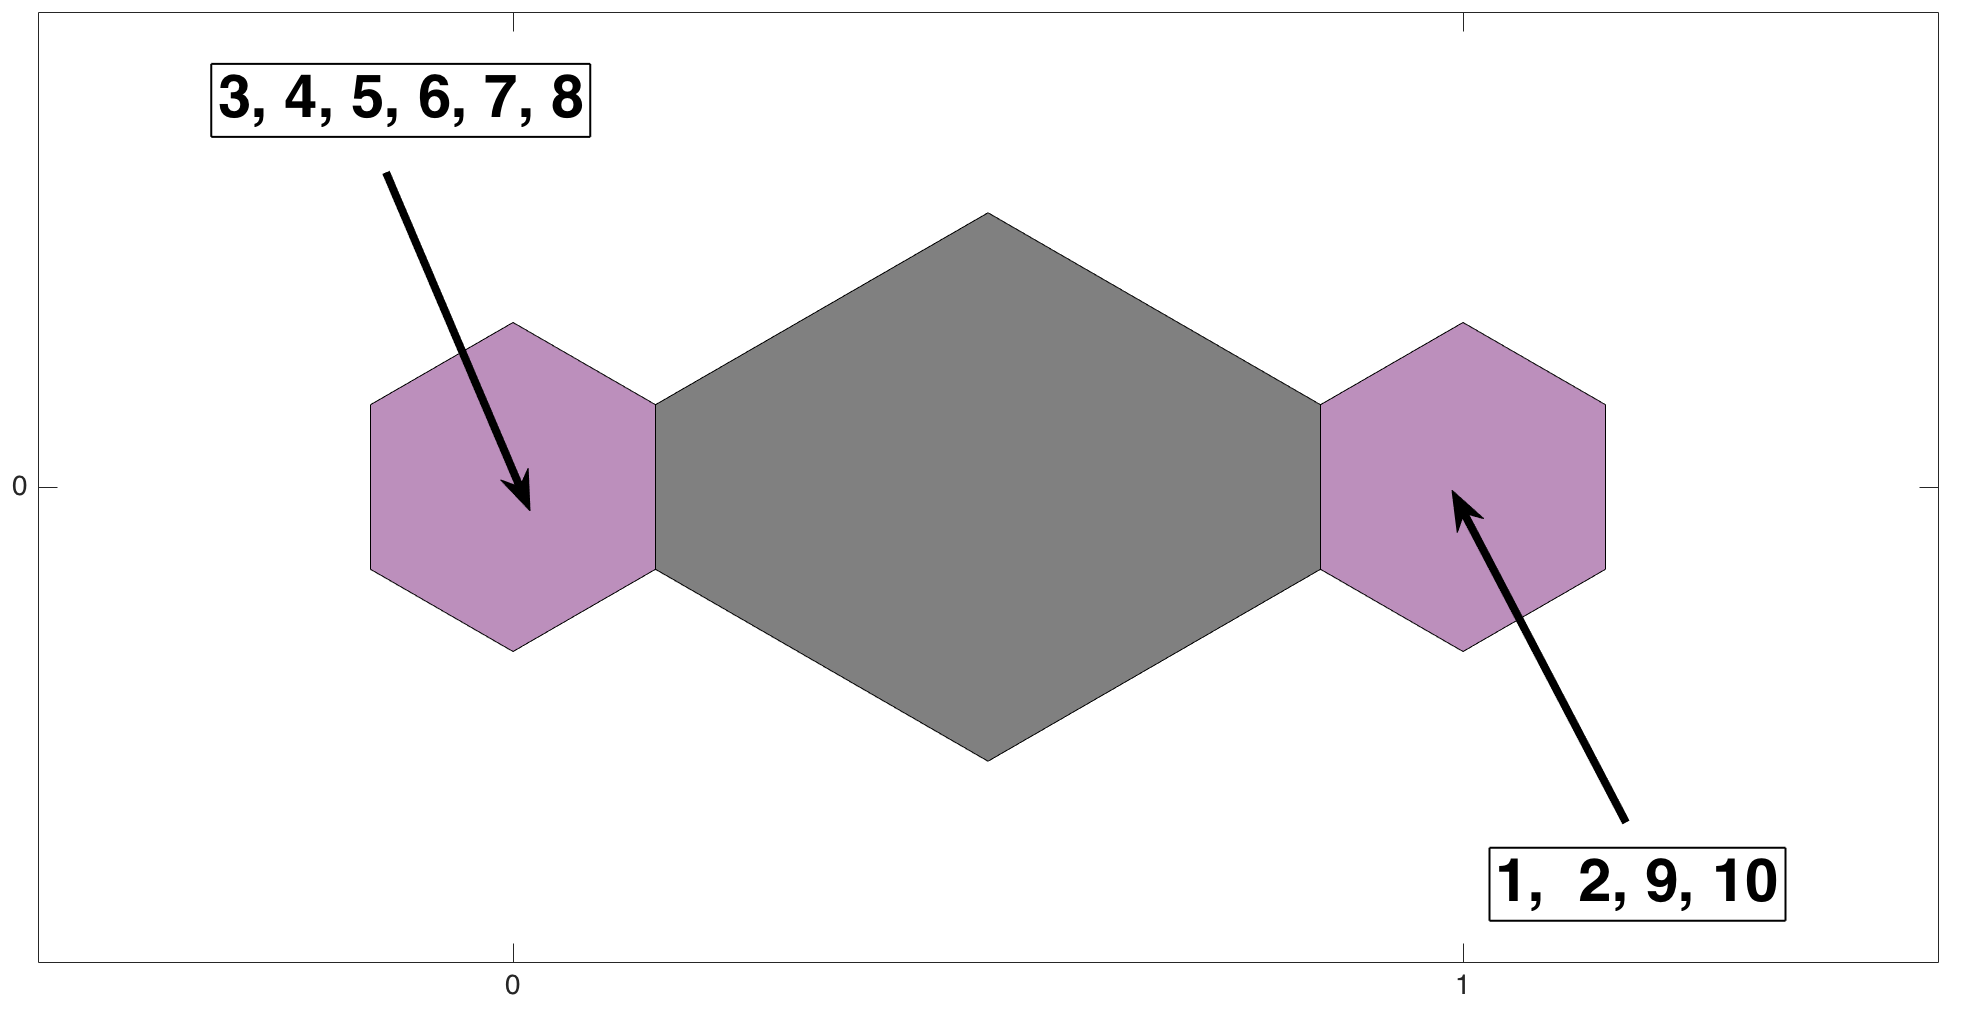
\includegraphics[width=0.5\textwidth]{../images0.01/M31/1D/combine_1D_1by2_all.png}
             }
            \hfill
            \subfloat[$1\times3$~network\label{fig: M31_net_1by3}]{
            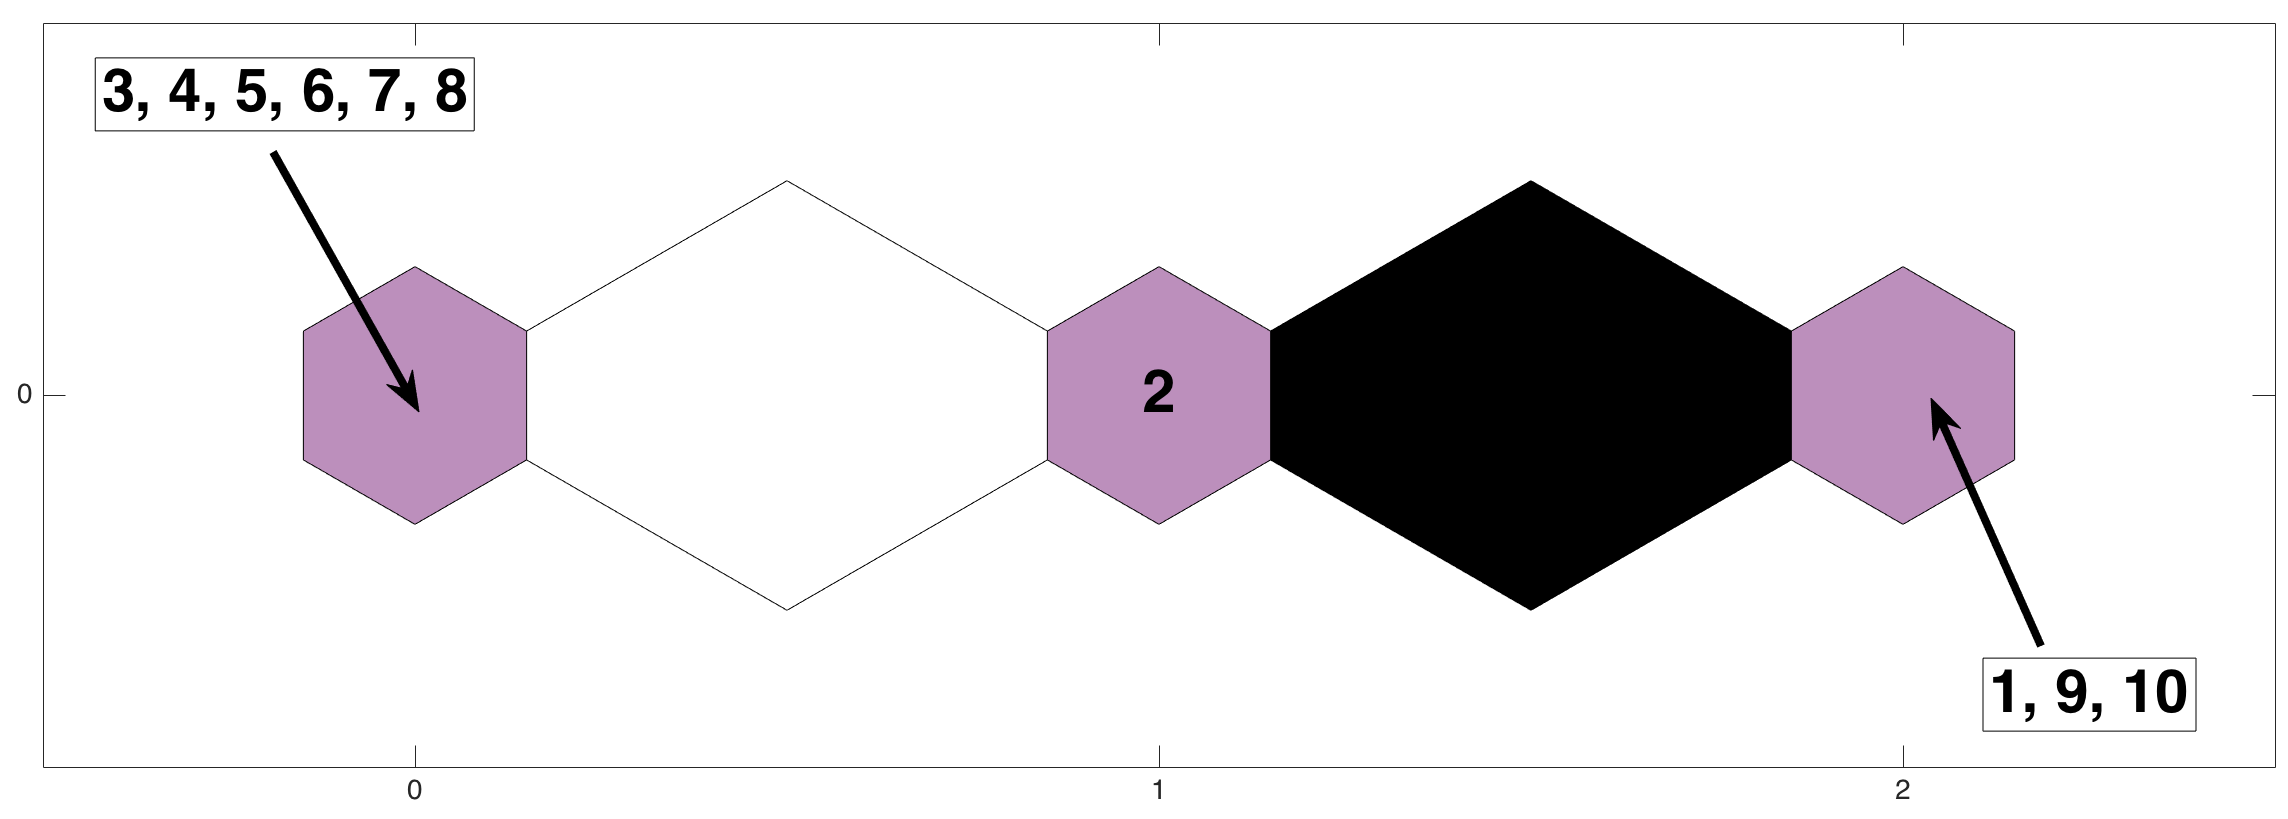
\includegraphics[width=0.5\textwidth]{../images0.01/M31/1D/combine_1D_1by3_all.png}
             }
             \hfill
            \subfloat[$1\times14$~network\label{fig: M31_net_1by14}]{
             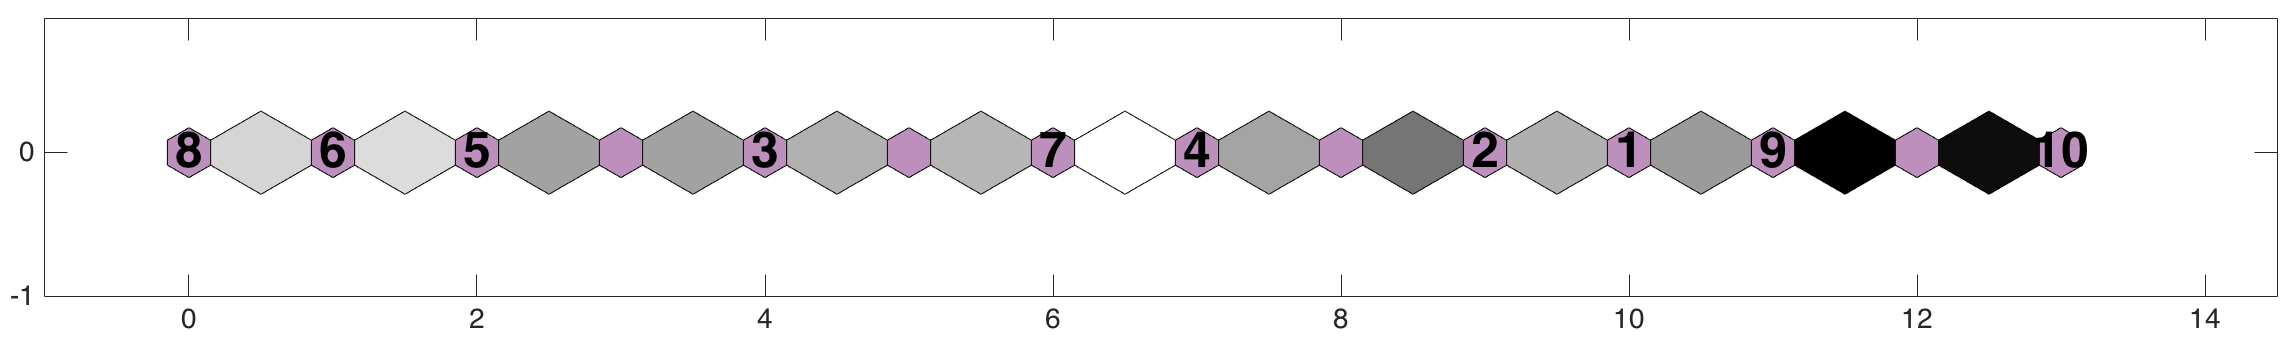
\includegraphics[width=0.5\textwidth]{../images0.01/M31/1D/combine_1D_1by14_all.png}
             }%%% What should I do with this one! It doesn't look good visually
            \caption{SOM of the M31 data from $1\times2$, $1\times3$~and $1\times14$~grids. The axes show the position of the neurons. The purple hexagonal shapes represent the neurons. The grey scale colours show the differences between weight of the neurons, with white as the minimum difference and black as the maximum. The numbers in the plot show the M31 regions located in each neuron.}
            \label{fig: M31_nets_1d}
        \end{figure}
        
        %%Network 1by14
        The network with 14 neurons, in Fig.~\ref{fig: M31_net_1by14}, is the first network that has no neuron occupied by more than one M31 region.
        In a larger-grid SOM, the network pays more attention to smaller details and differences in the input data.
        Therefore, since at least 14 neurons are needed to separate all 10 regions in M31, we can conclude that some of the regions have very small differences.
        Regions that are located in similar areas in M31, like region 7 and 4 (see Fig.~\ref{fig: regions in m31}), are most likely to show more similarities to each other.
        In Fig.~\ref{fig: M31_net_1by14}, the right-most neuron is occupied by region 10.
        Two black colours between this region and the others indicate the large differences between this neuron and the other ones.
       Region 10 is located in the bulge of M31, and its separation from other regions, which are mostly located around the inner or outer rings.
       The SOM shows that this region has a completely different input values than the others.
       Comparing raw data for regions shows that most of the input values for region 10 are much higher than the other regions, which is the main reason of its isolation.
        The region 8 occupies the right-most neuron in this network, suggesting that this region has the most differences from region 10.
        
        
    \subsection{Inside the 2 neuron network}%%% I will find better title for this subsection
        %What is going on in this section
        \label{sec: inside_the_2_neurons}
        Using self-organizing maps, we can identify hidden subgroups in our samples. 
        Each of these subgroups were separated from each other for a reason.
        This reason can vary from having higher values in some specific properties, as discussed in Sec.~\ref{Sec: 1d_cluster}, to some unknown correlations between data that cannot be seen in other groups or in the galaxy as a whole.
        To investigate the latter, we show in Fig.~\ref{fig: cor_cluster1} the Pearson correlation coefficients for the inputs from regions 3 to 8, which were clustered together in the $1\times2$ and $1\times3$ networks (see Figs.~\ref{fig: M31_net_1by2} and ~\ref{fig: M31_net_1by3}).
        
        \begin{figure}
        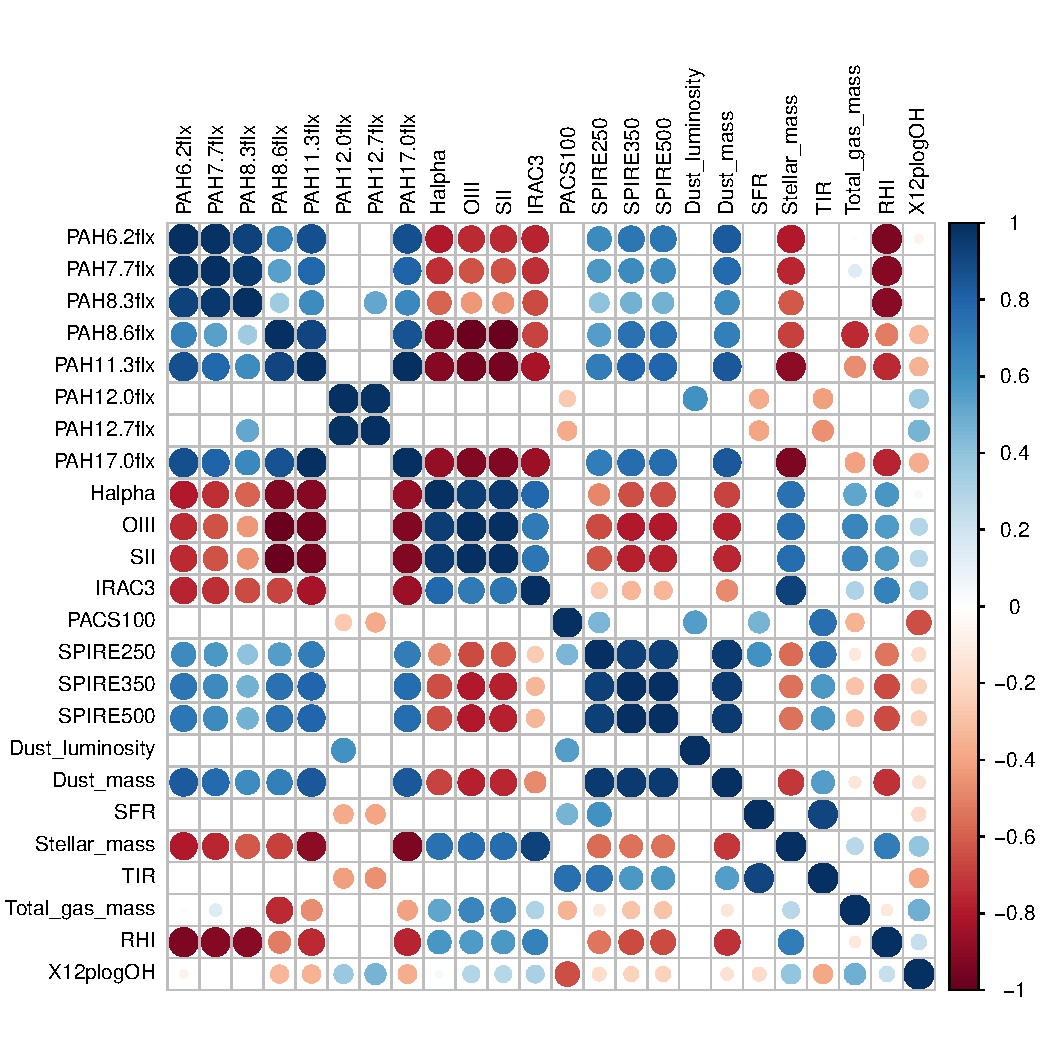
\includegraphics[width=0.5\textwidth]{../images0.01/cor_plots/M31_derived_3_to_8_core_plot_for_paper.pdf}%%% cut the white regions around the figure
        \caption{Same as Fig.~\ref{fig: cor_all}, but here we used data from regions grouped in the left sides of Figs.~\ref{fig: M31_net_1by2} and ~\ref{fig: M31_net_1by3}. }
          \label{fig: cor_cluster1}
        \end{figure}
        
        %%% what regions' version shows and how it compares with the other one:
        In Fig.~\ref{fig: cor_all}, which shows the Pearson correlation coefficients from data in all 10 regions, all the PAH features are highly correlated with each other. 
        Also, there are very strong correlations between all the PAH features and PACS~100~$\mu$m~, SPIRE 250 to 500~$\mu$m~emission, L$_{\rm dust}$, L$_{\rm TIR}$, SFR, and metallicity.
        However, in Fig.~\ref{fig: cor_cluster1}, the 12.0 and 12.7~$\mu$m~PAH fluxes do not show any significant or strong correlation with PAH fluxes in other wavelengths, or with most of the other quantities.
        The only exceptions are the strong correlations between PAH flux at 12~$\mu$m and L$_{\rm dust}$, and between the 12 and 12.7~$\mu$m PAH fluxes.
        Since there are only 6 regions in this cluster, even one outlier in the data may cause the correlation coefficient to become insignificant.
        If we ignore the outlier values, the correlations between 12.0 and 12.7~$\mu$m~PAH fluxes and the other quantities show themselves. 
        For example region 8 breaks correlations between 12.0~$\mu$m and 6.2, 7.7, and 8.3~$\mu$m.
        This region could be part of scatter for these correlations, but with 6 regions in the dataset it is hard to have a concrete conclusion.
        
        For the remaining PAH fluxes in Fig.~\ref{fig: cor_cluster1}, there are no significant correlations with PACS~100~$\mu$m, L$_{\rm dust}$, L$_{\rm TIR}$, SFR, or metallicity.
        These fluxes correlate with SPIRE emission, but to a lesser extent than for data from all regions.
        Correlations between PAH features and SFR, and L$_{\rm TIR}$ are well-studied~\citep[e.g.][]{Tielens08,Peeters04}. 
        Many groups have used PAH features as a tracer of SFR by finding correlations between 
        PAH emission and SFR derived from extinction-corrected \halpha~\citep[e.g.][]{Shipley16,Khramtsova13,Calzetti07}.
        These correlations are seen in Fig.~\ref{fig: cor_all}, when we considered the data from all regions, but not in Fig.~\ref{fig: cor_cluster1} when considering the clustered data.
        Further analyses show that the absence of correlations between PAH fluxes and SFR, is because of one outlier: Region 6. 
        When we disregard this region, high correlations between 6.2 to 11.3~$\mu$m~PAHs and SFR (and L$_{\rm TIR}$) reappear.
        Strong anti-correlations between 6.2 to 11.3~$\mu$m~PAH features and RHI, stellar mass, \halpha, \sii, \oiii, and IRAC~5.6~$\mu$m~emission in Fig.~\ref{fig: cor_cluster1} were not seen in Fig.~\ref{fig: cor_all}.
     
        Anti-correlations between PAH features and the \halpha, \sii, and \oiii~emission could be the result of one of the following. 
        First, the optical data are not corrected for dust extinction.
        The PAH features correlate with the amount of dust while \halpha~emission anti-correlates with amount of dust due to extinction \citep{Calzetti94}.
        Therefore, higher PAH fluxes imply higher dust abundance and less \halpha~emission, and the same for \sii~and \oiii~emission.
        Second, is the possible effect of observing apertures.
        If the observed regions are located near the edge of H {\sc II} regions we would expect to see more PAH and less \halpha~emission. %%% reference? PB: I will try to find one.
        The anti-correlations between 6.2 to 11.3~$\mu$m~PAH features and RHI have been seen in other studies, as well~\citep[e.g.][]{Dim15, Gordon08, Wu06}.
        \cite{Wu06} suggested these anti-correlations could be the result of PAH destruction due to a high amount of harder radiation (thus higher RHI).
        On the other hand, \cite{Gordon08} argued that the harder radiation could make the photodissociation regions (PDRs) smaller.
        The PAH features are mostly coming from the PDRs that are surrounded by H {\sc II} regions, and the PAH features' underlying continuum emission is from the H {\sc II} regions.
        Therefore, the lower flux of the PAH features could be the result of the smaller size of PDRs.
        The later reason, which could also describe the anti-correlation between PAH features and \halpha~emission, seems to be the more probable one. 
        
        The strong anti-correlation between PAHs and stellar mass suggests that, despite the general assumption that one of the main source of heating PAHs is stellar emission~\citep[e.g][]{Haas02,Bendo08,Calapa14, Lu14,Jones15}, a higher stellar mass decreases PAH emission.
        In observations of M33,~\cite{Calapa14} showed that the 8/250~$\mu$m luminosity ratio correlates with 3.6~$\mu$m emission, which translates to stellar mass, and conclude that the PAH emission traces the old stellar population.
        In Fig.~\ref{fig: cor_cluster1}, we see a weak anti-correlation between SPIRE 250~$\mu$m emission and the stellar mass.
        We see no correlation between 8/250~$\mu$m luminosity and stellar mass, either in clustered data or in all 10 regions.
      %  The results from~\cite{Calapa14} were based on data from the whole galaxy and has a relatively high scatter.
      %It is possible that all the 10 regions in M31 simply aligned with the scatter of the correlation. Further analysis on M31 data is required to see weather the anti-correlation in this regions is extended to whole galaxy or it is only for these 6 regions.
        
        Some studies have indicated that strong stellar emission could lead to destruction of PAHs ~\citep[e.g.][]{Clayton03,Seok14}.
        To test that whether anti-correlation between stellar mass and PAH emission is the result of the destruction of PAHs in high stellar mass regions, or that high stellar mass obscures PAH emission, we compared PAH abundance with stellar mass for the clustered regions.
        The ratio of 8/24~$\mu$m emission, which can be considered as a proxy for PAH abundances~\citep[e.g.][]{Sandstrom10,Khramtsova13}, does not anti-correlate with stellar mass for either the clustered data or all 10 regions.
        Therefore, we conclude that in our sample,  stellar mass does not cause the destruction of PAHs.
        
        The anti-correlation between stellar mass and PAHs could be result of the position of the regions in M31.
        Regions 5, 6, and 8 are located on the stellar disk of the galaxy and have relatively high stellar mass and low PAHs. 
        According to~\cite{Dim15}, regions 5 and 8 are the only two regions in our sample that do not include an H {\sc II} region, which could be the reason of low PAHs for these regions.
        Regions 4 and 7 have similar quantities for both stellar mass and PAHs and region 3 has high PAHs and low stellar mass.
        Without data from more regions in M31, we cannot confidently say that higher stellar mass decreases PAH fluxes.
        %% Sahar: Can we have higher PAHs absorbes stellar mass and thats why we see the anti-correlation?!!!
        
       % On the other hand, if we divide SFR by stellar mass, which give us specific star formation rate (sSFR), we see strong correlation between sSFR and 6.2 to 11.3~$\mu$m fluxes for clustered regions,
        
        
       Regardless of the fact that some of the (anti)-correlations in Fig.~\ref{fig: cor_cluster1} might have physical meaning, we have to mention that we only used 6 regions to calculate these correlation coefficients.
       The number of data points is not high enough to yield a strong conclusion about PAH properties in M31.%%% it doesn't sound right:((
        However, we can conclude that since the correlation coefficients derived from the clustered data (Fig.~\ref{fig: cor_cluster1}) differ from the correlation coefficients derived from the data from the all regions (Fig.~\ref{fig: cor_all}), the SOM separated a hidden cluster of the data which has different properties. %%Again eh!
        
        
        
        
        
